\documentclass[a4paper]{article}
\usepackage{amsmath}
\usepackage{xcolor}
\usepackage{amsthm}
\newtheorem{thm}{Theorem}
\usepackage[english]{babel}
\usepackage[utf8]{inputenc}
\usepackage{graphicx}
\usepackage[colorinlistoftodos]{todonotes}

\title{\textbf{Cell Energetics}}
\author{Abhiraj Mallangi}
\date{Chapters 6 \& 8, \textit{Campbell Biology in Focus}}
\begin{document}
\maketitle

\tableofcontents
\newpage

\section{Metabolism}
The totality of an organism's chemical reactions is called \color{red} metabolism\color{black}, which manages the material and energy resources of the cell.\\

A \color{red}metabolic pathway \color{black} is a series of chemical reactions that either builds a complex molecule or breaks down a complex molecule into simpler molecules, and a specific enzyme catalyzes each step (see Figure 1).

\begin{itemize}
	\item Catalysts are substances that increase or decrease the rate of a chemical reaction but remain unchanged.
	\item Enzymes are \underline{proteins} that increase the rate of chemical reactions by converting a substrate into a product, and \underline{are also catalysts}.
		\begin{itemize}
			\item Prote\textit{ase} is an enzyme that breaks down proteins.
			\item Lip\textit{ase} is an enzyme that breaks down lipids.
			\item Carbohydr\textit{ase} is an enzyme that breaks down carbohydrates.
			\item Denaturalization reactions are those that change the shape of an enzyme by temperature or pH.
		\end{itemize}
\end{itemize}

\begin{figure}[h!]
\centering
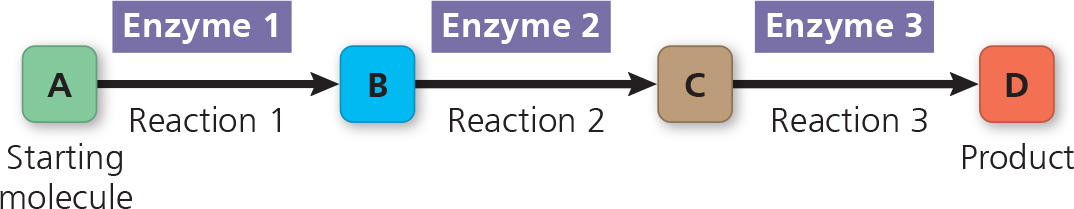
\includegraphics[width=0.7\textwidth]{figure_one.jpeg}
\caption{A representation of metabolic pathways.}
\end{figure}

\subsection{Catabolic Pathways}
\color{red}Catabolic pathways\color{black}, or breakdown pathways, release energy by breaking down complex molecules into simpler molecules.

\begin{itemize}
	\item Cellular respiration, which breaks down glucose and other organic fuels, is a major catabolic pathway.
\end{itemize}

\subsection{Anabolic Pathways}
\color{red}Anabolic pathways\color{black}, or biosynthetic pathways, consume energy to build complicated molecules from simpler ones.

\begin{itemize}
	\item The synthesis of amino acids from simpler molecules and the synthesis of proteins from amino acids are anabolic reactions.
\end{itemize}

\section{Energy}
\color{red}Energy \color{black} is defined as \textbf{the capacity to cause change}.

\subsection{Forms of Energy}
\begin{itemize}
	\item \color{red}Kinetic Energy \color{black} is that associated with the relative motion of objects.
		\begin{itemize}
			\item Thermal energy is a type of kinetic energy associated with the random \textit{movement} of atoms or molecules.
		\end{itemize}
	\item \color{red}Potential energy \color{black} is that of an object not presently moving, the energy matter possesses because of its location or structure.
		\begin{itemize}
			\item Chemical energy, necessary for an organism's survival, is that stored in bonds, released when molecules rearrange such that the potential energy is converted to kinetic energy, and is frequently measured in calories.
		\end{itemize}
\end{itemize}

\subsection{Thermodynamics}
\color{red}Thermodynamics \color{black} is the study of energy transformations that occur in a collection of matter.
\begin{itemize}
	\item A \textit{system} is used to denote the matter under the study.
	\item \textit{Surroundings} is used to refer to everything outside the system.
	\item An \textit{isolated system}, is that unable to exchange either energy or matter with its surroundings.
	\item An \textit{open system} is that where energy and matter can be transferred between the system and its surroundings.\\
\end{itemize}

\color{red}The First Law of Thermodynamics \color{black} states that \textbf{energy can be transferred and transformed, but it cannot be created or destroyed}, and is also known as the \textit{principle of conservation of energy}.

\begin{itemize}
	\item Ultimately, all energy \textit{decomposes} into thermal energy, heat.
	\item Reactions \textit{rearrange} atoms, but do not destroy them.
\end{itemize}

\color{red}The Second Law of Thermodynamics \color{black} states that \textbf{energy transfer or transformation increases the entropy of the universe}.
\begin{itemize}
	\item \color{red}Entropy \color{black} is a measure of molecular disorder, or randomness. The more randomly arranged a collection of matter is, the greater its entropy, and the more organized a collection of matter is, the lesser its entropy.
		\begin{itemize}
			\item Greater entropy releases energy, and lesser entropy absorbs energy. 
			\item Because greater entropy releases energy, the universe tends to want greater entropy.
		\end{itemize}
\end{itemize}

\subsection{Endothermic \& Exothermic Reactions}

\color{red}Endothermic reactions \color{black} are those that \textit{absorb} energy. 
\color{red}Exothermic reactions \color{black} are those that \textit{release} energy.\\

A \color{red} spontaneous process \color{black} is one such that, by itself, it leads to an increase in entropy or can proceed without requiring an input of energy. A \color{red} nonspontaneous reaction \color{black} is one such that it leads to a decrease in entropy and can only proceed if energy is supplied.

\subsection{Free Energy}
\color{red}Free energy \color{black} is the portion of a system's energy that can perform work when temperature and pressure are uniform throughout a system. $\Delta G$ represents the difference between the free energy of the final state and the free energy of the initial state such that $$\Delta G = G_{\text{final state} - G_{\text{initial state}}} $$

\begin{itemize}
	\item Endothermic reactions have a positive $\Delta G$ (see Figure 2).
	\item Exothermic reactions have a negative $\Delta G$ (see Figure 2).
\end{itemize}

\begin{figure}[h!]
\centering
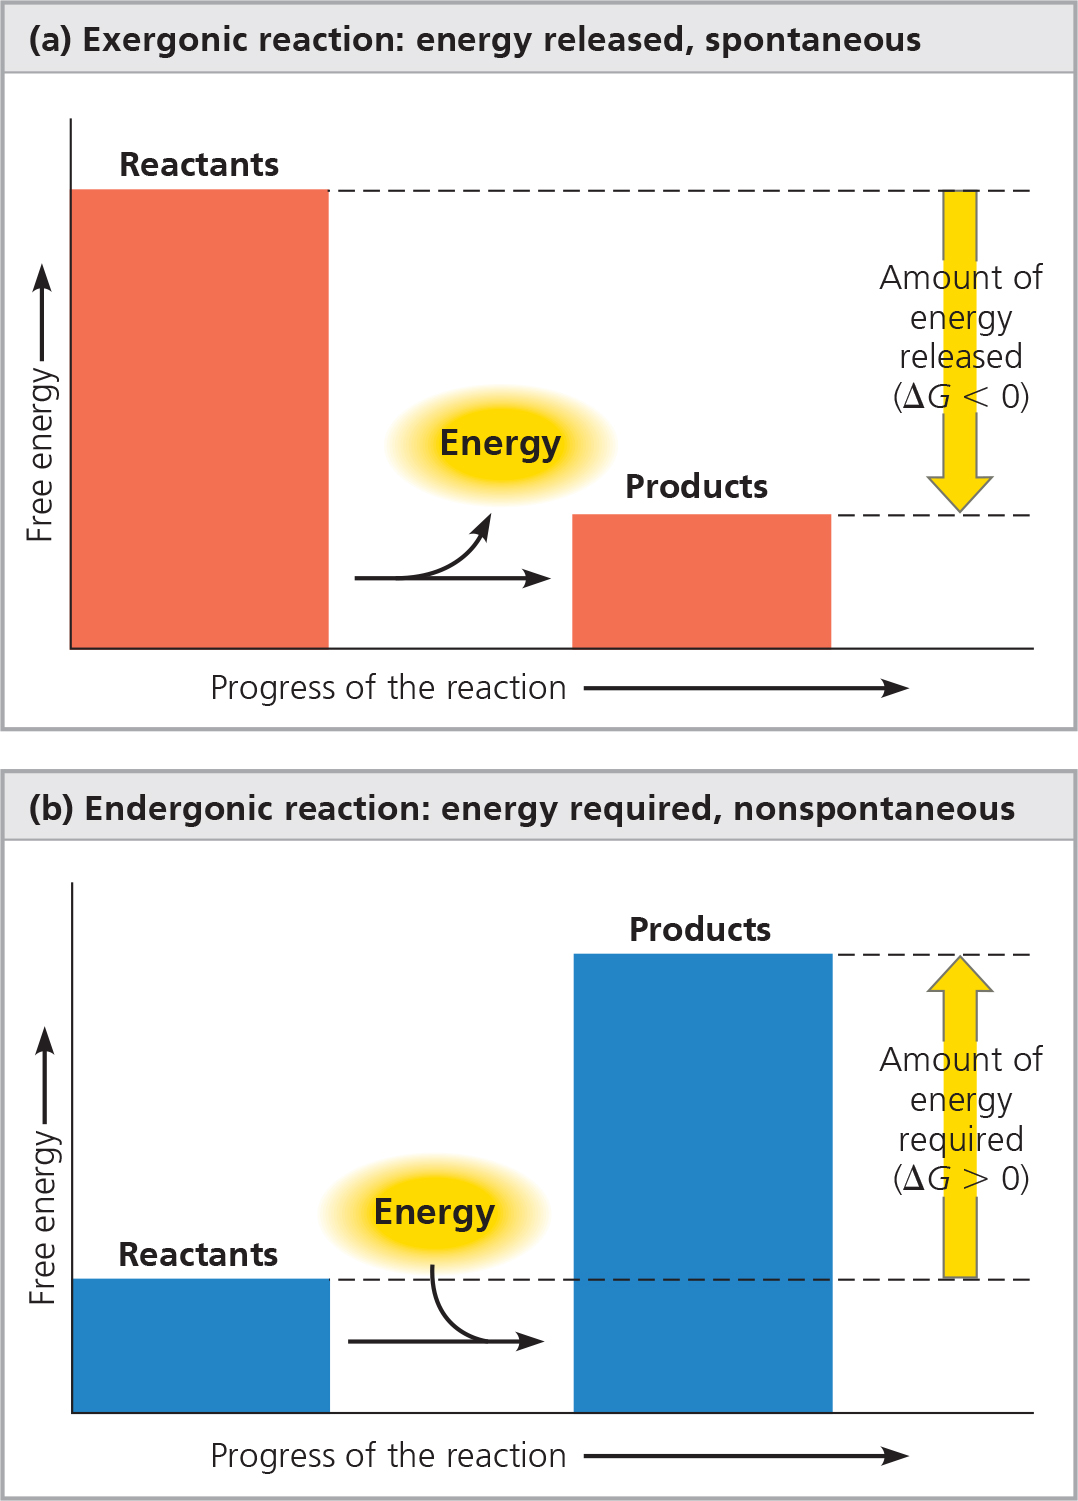
\includegraphics[width=0.7\textwidth]{figure_two.jpeg}
\caption{Here, endergonic refers to endothermic, and exergonic refers to exothermic.}
\end{figure}

\color{red}Equilibrium \color{black} is a state of maximum stability, the forward and reverse reactions occur at the same rate, and there is no further net change in the relative concentration of products and reactants. When a system reaches equilibrium, it is at its lowest $|\Delta G|$ (see Figure 3). For instance, cells reach equilibrium when they die because energy fails to move into and out of the cell, it remains constant.

\begin{figure}[h!]
\centering
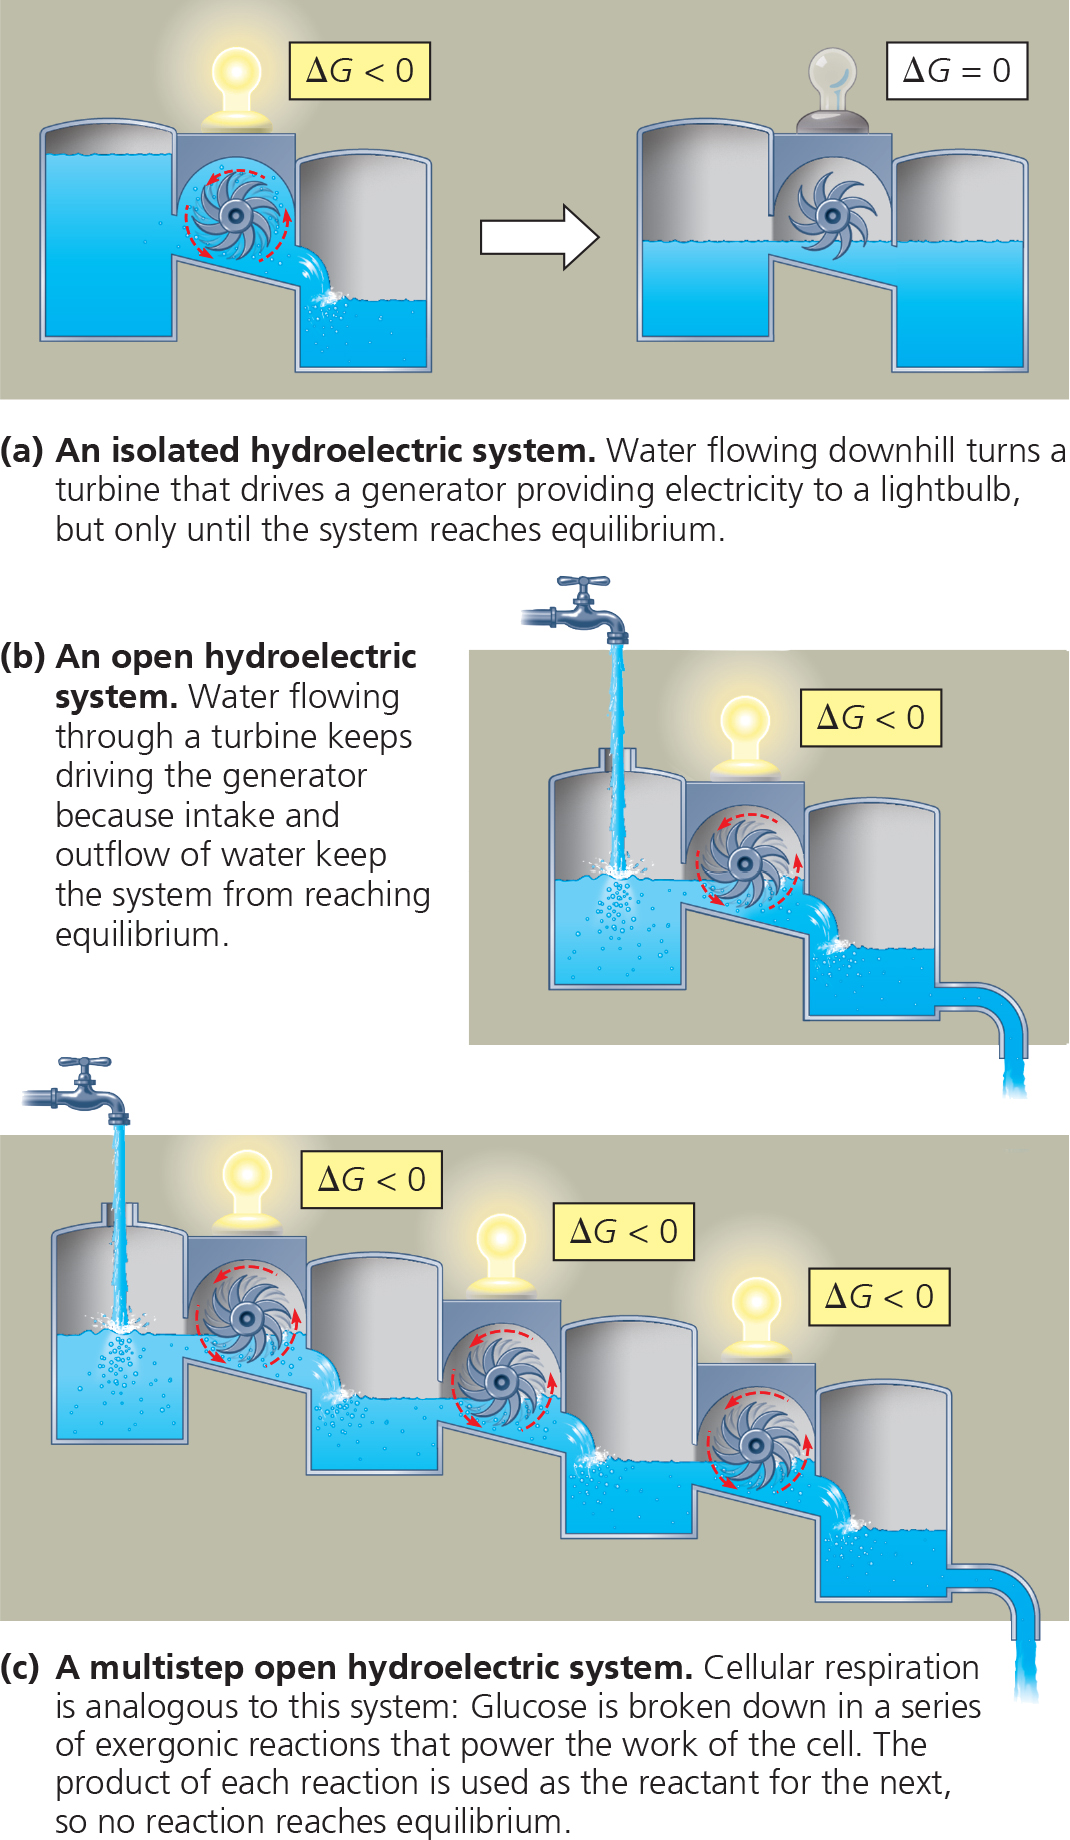
\includegraphics[width=0.7\textwidth]{figure_three.jpeg}
\caption{The illustrations demonstrate how a system reaches its lowest $\Delta G$, or equilibrium.}
\end{figure}

\section{Adenine Triphosphate (ATP) \& Energy Coupling}
A cell does three main kinds of work:
\begin{itemize}
	\item \textit{Chemical work}, the pushing of exothermic reactions that would not occur spontaneously, such as the synthesis of polymers from monomers.
	\item \textit{Transport work}, the pumping of substances across membranes against the direction of spontaneous movement.
	\item \textit{Mechanical work}, such as the beating of cilia, the contraction of muscle cells, and the movement of chromosomes during cellular respiration.
\end{itemize}

Cells use \color{red}energy coupling\color{black}, the use of energy released from an exothermic reaction to drive an endothermic reaction, to manage their energy resources.\\

\subsection{ATP Structure}
\color{red}ATP \color{black} is a compound containing the sugar ribose, the nitrogenous base adenine, and a chain of three phosphate groups attached to it (see Figure 4).

\begin{figure}[h!]
\centering
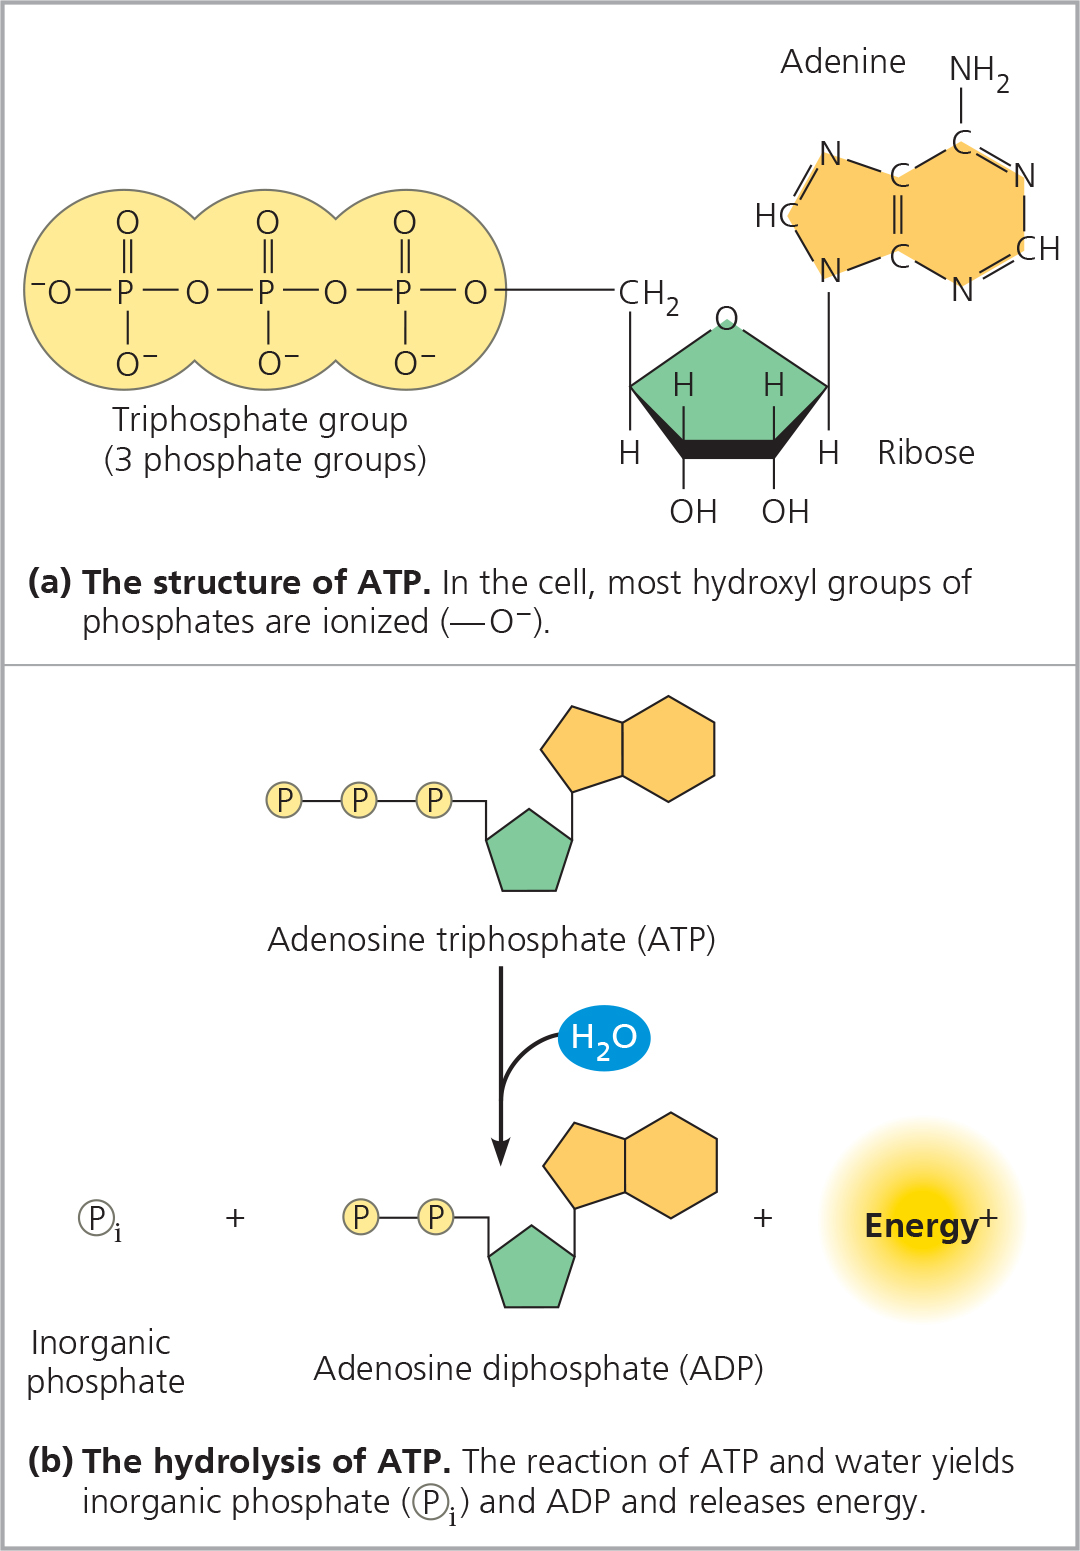
\includegraphics[width=0.7\textwidth]{figure_four.jpeg}
\caption{The illustrations show ATP structure.}
\end{figure}

\subsection{ATP Hydrolysis}
When the bonds between ATP phosphate groups are broken by hydrolysis, a molecule of inorganic phosphate, ${\text{HOPO}_3}^{2-}$ leaves the ATP. This exothermic reaction releases $7.3$ kcal of energy per mole of ATP hydrolyzed. In addition, in cellular conditions, this exothermic reaction releases $13$ kcal of energy per mole of ATP.\\

\subsection{Energy Coupling \& Work}
For energy coupling to occur, the broken-off phosphate group must bond to another molecule, now called a \color{red}phosphorylated intermediate\color{black}. Sometimes this causes a shape-change that allows \textit{mechanical work}.

\subsection{ATP Regeneration}
An organism at work uses ATP continuously, but ATP is a renewable resource that can be regenerated by the addition of phosphate to ADP, the \textit{ATP Cycle} (see Figure 5).

\begin{figure}[h!]
\centering
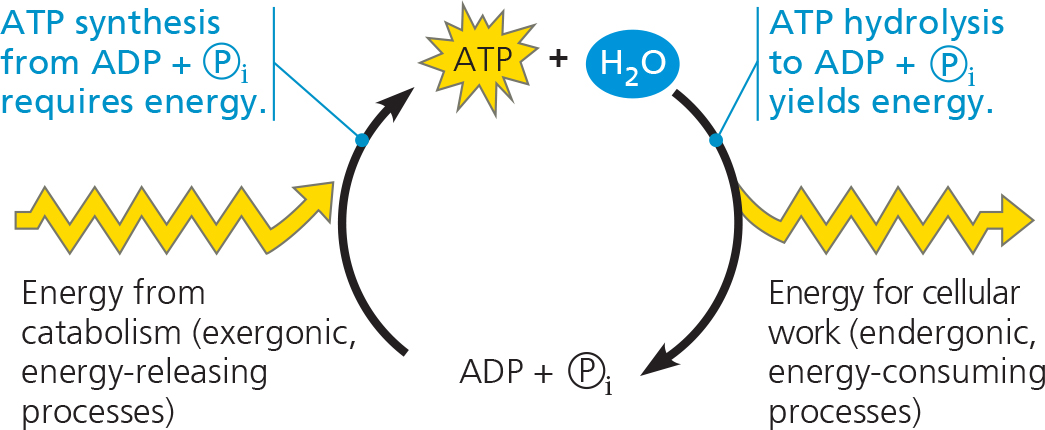
\includegraphics[width=0.7\textwidth]{figure_five.jpeg}
\caption{The illustrations demonstrate ATP regeneration.}
\end{figure}

\section{Photosynthesis}
\color{red}Photosynthesis \color{black} is the remarkable ability of an organism to harness light energy and use it to drive the synthesis of organic compounds. Photosynthesis emerges from the structural organization of the cell, when photosynthetic enzymes and other molecules are grouped together in a biological membrane, enabling the necessary series of chemical reactions to be carried out efficiently.

\subsection{Photons}
Photons are packets of light energy, and each type of photon has a \textit{fixed} amount of energy. Light, consisting of photons, moves as a \textbf{wave} (see Figure 6).

\begin{figure}[h!]
\centering
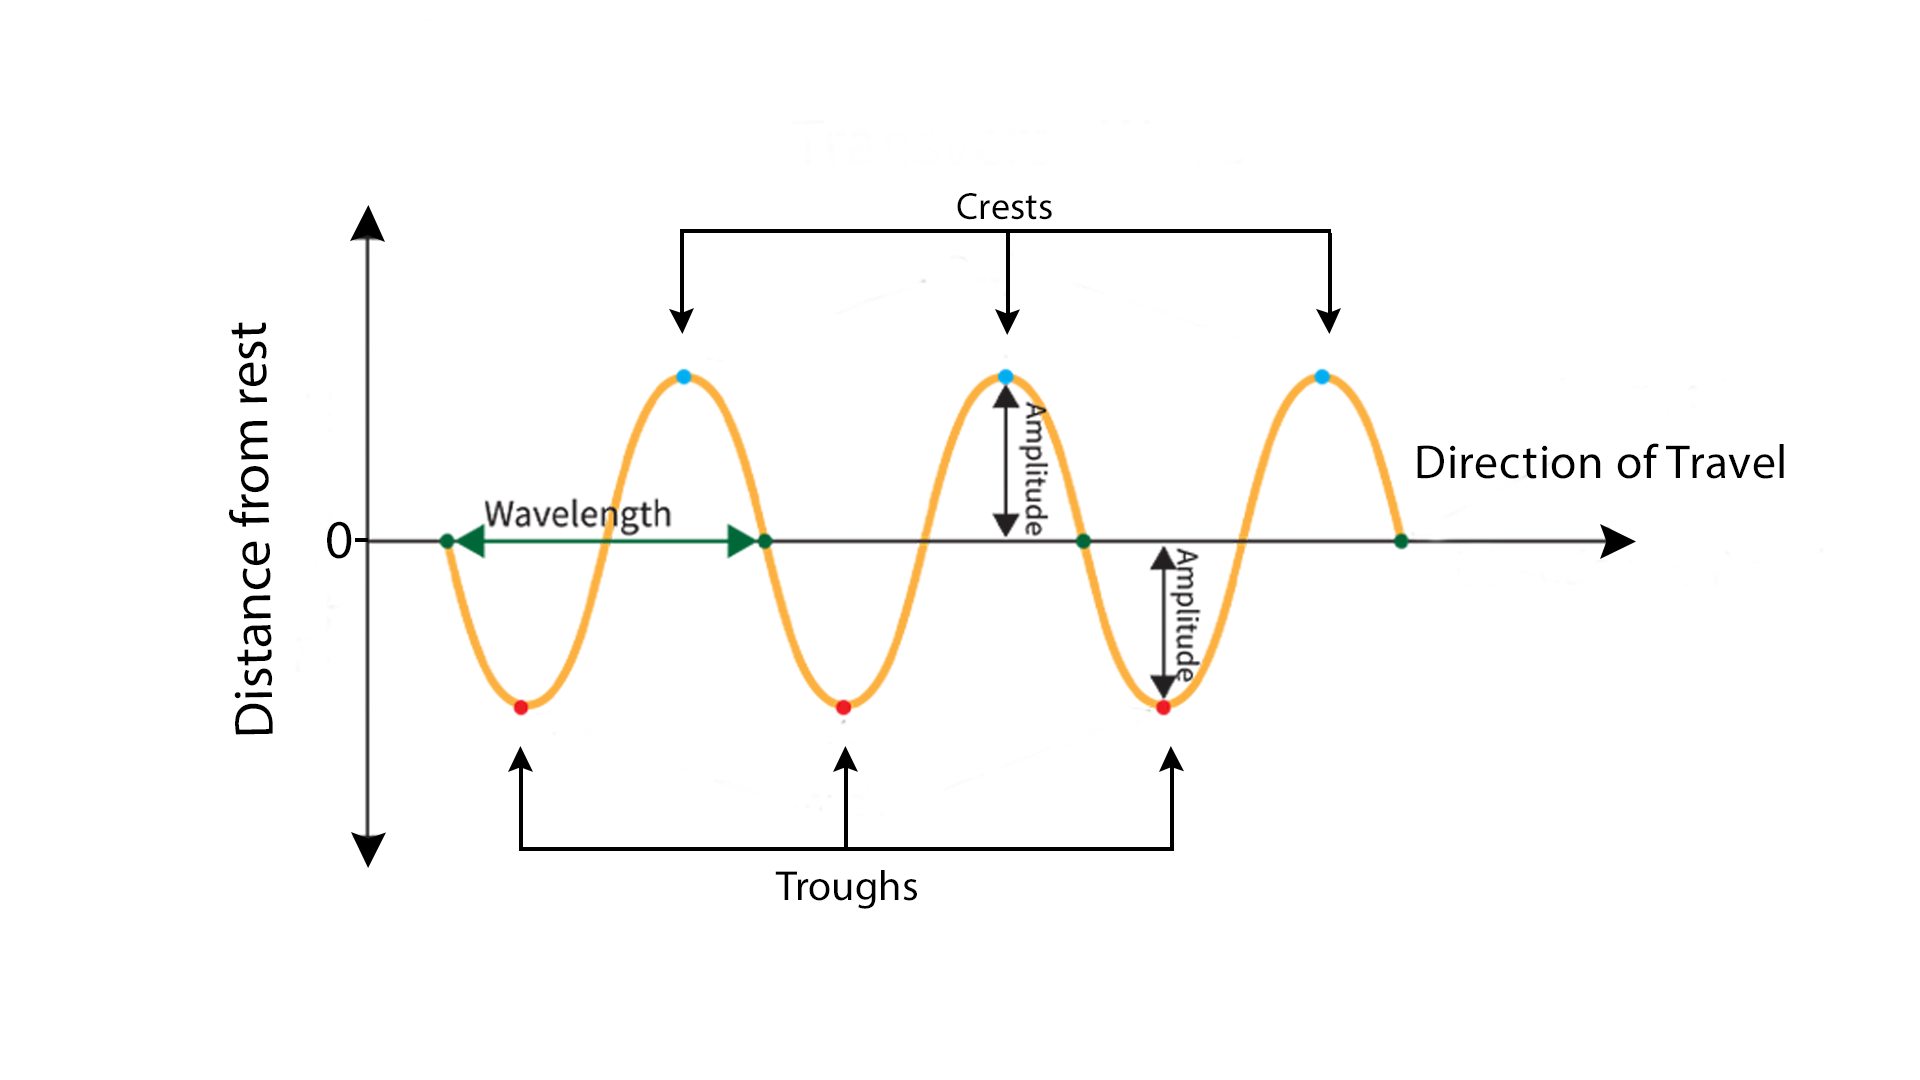
\includegraphics[width=0.7\textwidth]{figure_six.png}
\caption{The illustration represents the features of a wave.}
\end{figure}

The electromagnetic spectrum is a chart that shows the different types of radiation that stems from the sun (see Figure 7).

\begin{figure}[h!]
\centering
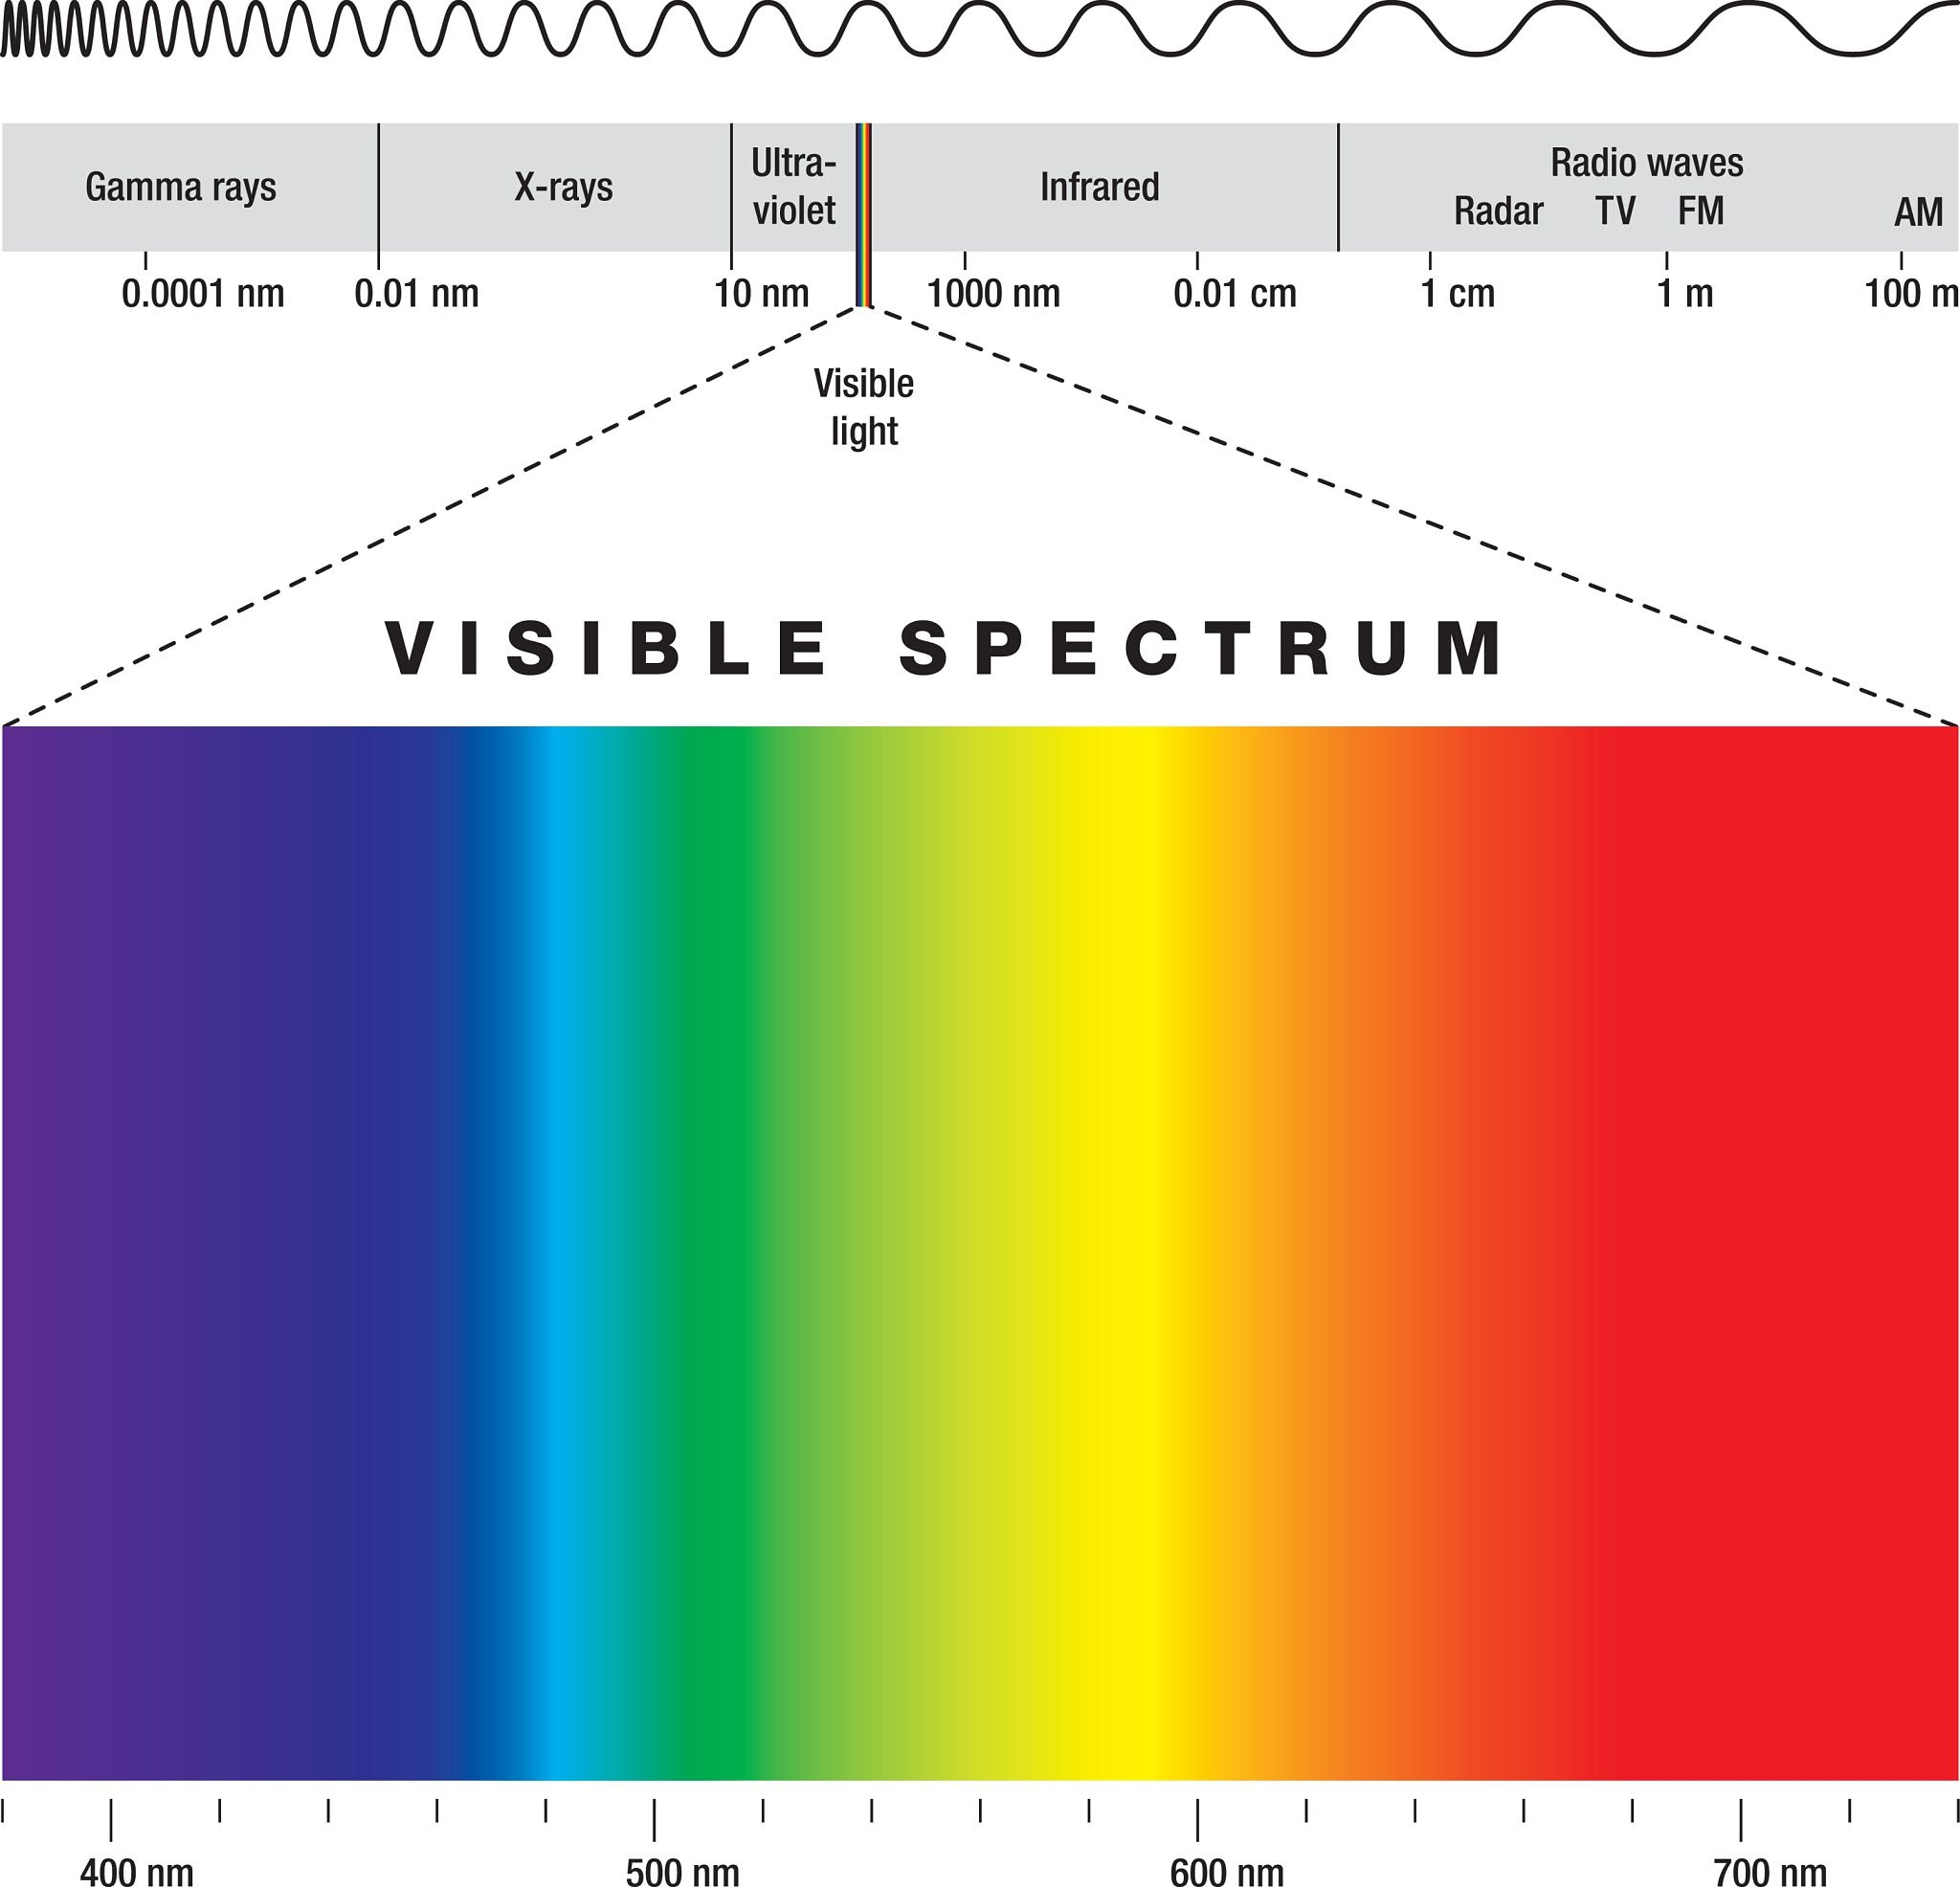
\includegraphics[width=0.5\textwidth]{figure_seven.jpeg}
\caption{From left to right, the wavelength and energy lessens. Across the \textit{visible light} range, we see differing colors.}
\end{figure}
\end{document}
